\chapter{Transition Metal Systems Benchmark}
\label{ch:benchmark}
\section{Introduction}
% \label{sec:benchmark:intro}
Most electronic structure computation studies use experimental data for comparison and assessment.
Since experimental observables are usually the differences between energies from theoretical models, many calculations could produce a good agreement to experiments by coincidence, or cancellations of errors, which are not well-examed.

In this project, we apply a set of electronic structure methods to a set of small realistic transition metal systems.
For each system, the Hamiltonian is carefully controlled to ensure all the methods are calculating exactly the same system with the same system-level approximations.
This approach allows us to access methodological differences directly with obfuscation from other errors.

The methods that we compare include self-energy embedding theory (SEED), auxiliary field quantum Monte Carlo (AFQMC), coupled cluster with singles, doubles and perturbative triples (CCSD(T)), full configuration interaction quantum Monte Carlo (FCIQMC), density matrix renormalization group (DMRG), fast semistochastic heat-bath configuration interaction (SHCI), configuration interaction with singles and doubles (CISD), second order Green function (GF2), coupled cluster with singles and doubles (CCSD), multireference linearized coupled cluster (MRLCC), quasi-particle self-consistent GW approximation (QSGW), Hartree-Fock random-phase approximation (HF+RPA),  self-consistent GW approximation (SC-GW), diffusion Monte Carlo with single determinant nodal surface (DMC(SD)), DFT in local density approximation (LDA), DFT in PBE approximation (PBE), DFT with HSE06 functional (HSE06), DFT with B3LYP functional (B3LYP), and DFT with SCAN functional (SCAN).

\section{Results}

We use SHCI results as the reference values for these systems.
The SHCI results are systematically converged to less than 1~mHa uncertainty.
Fig.~\ref{fig:benchmark} presents the results.

\begin{figure}
  \begin{center}
  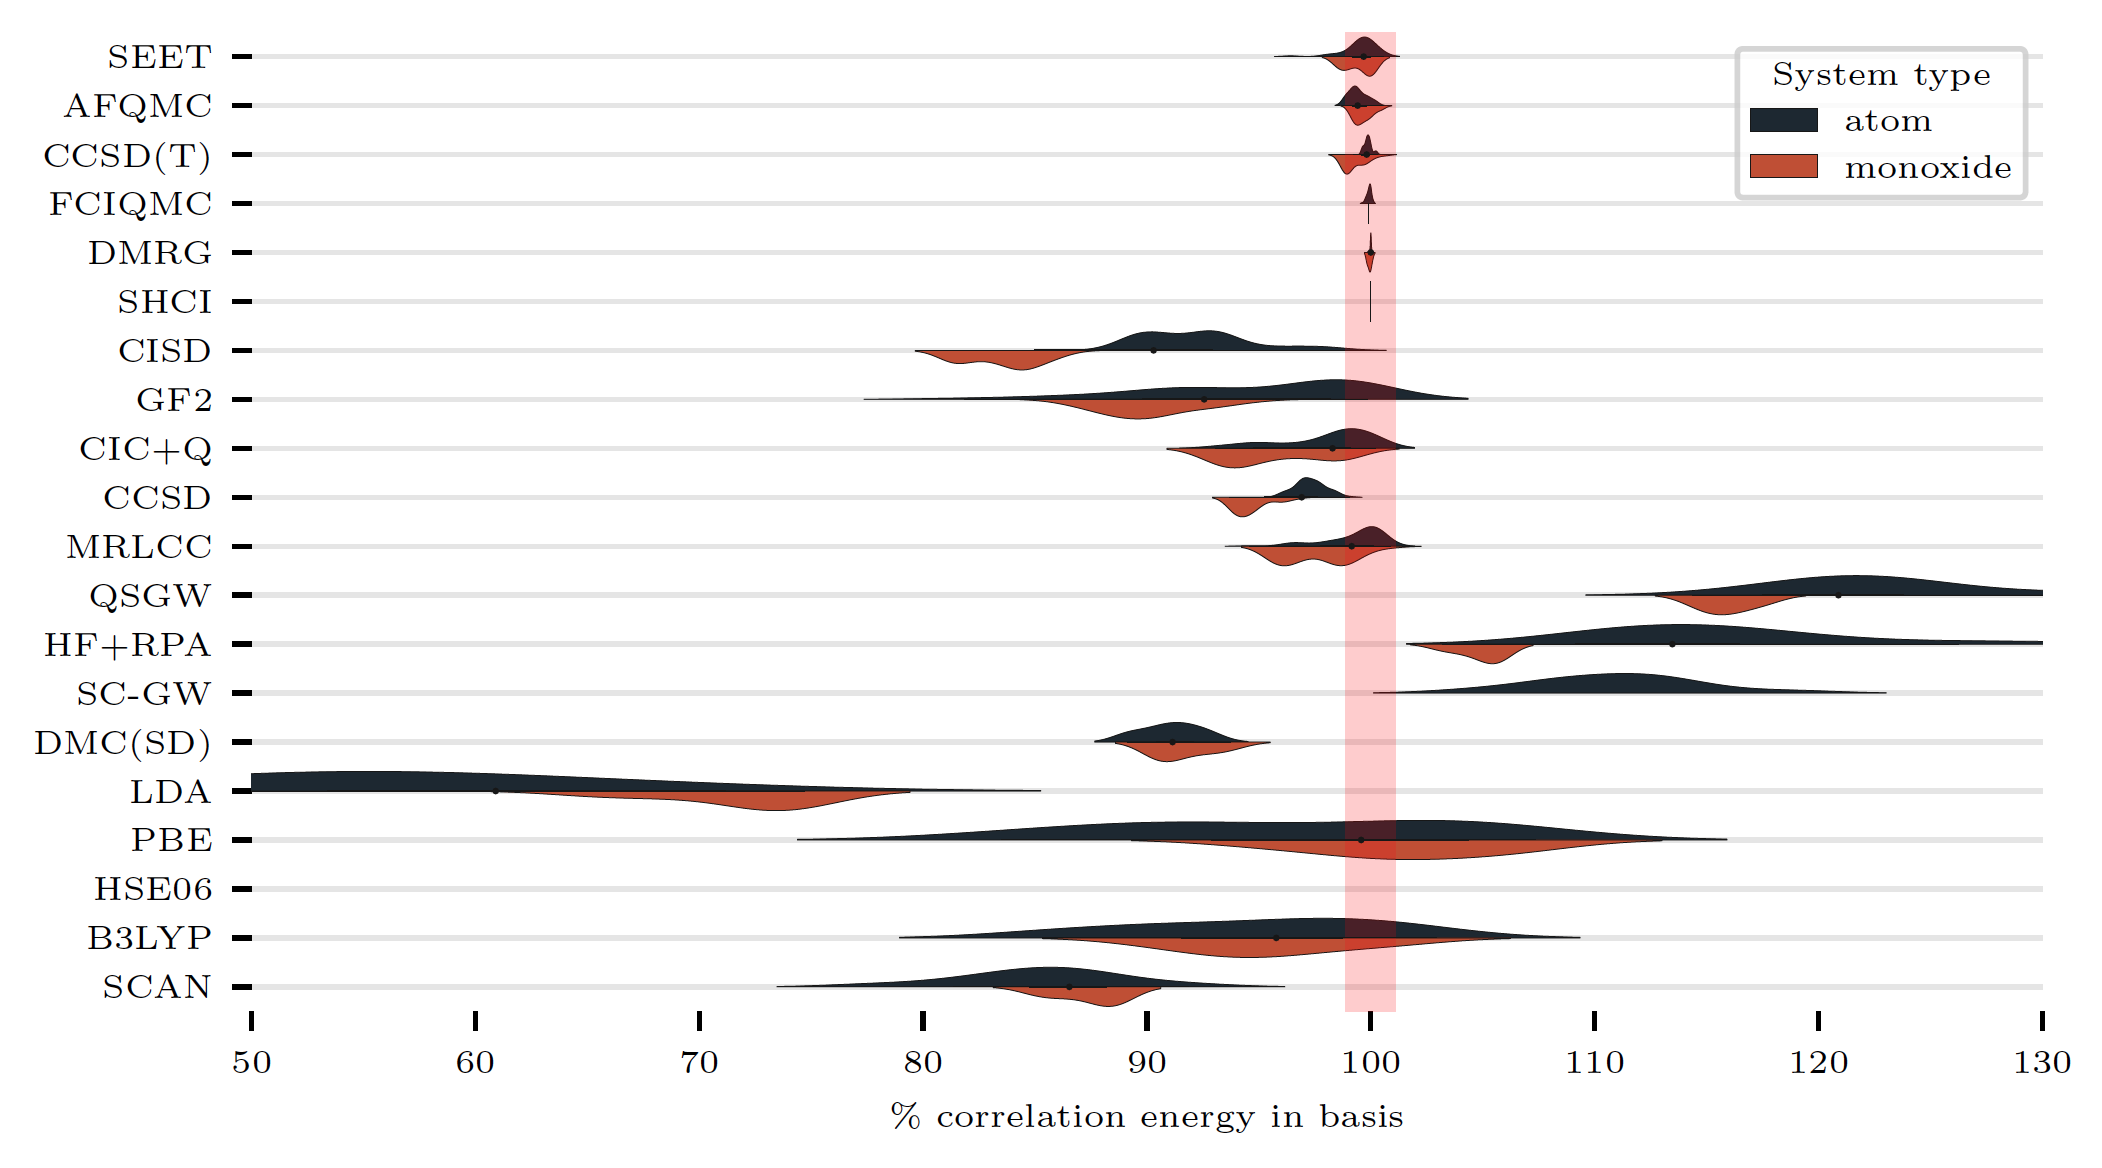
\includegraphics[width=\linewidth]{figs/benchmark.png}
  \caption{Percent of Correlation Energy Recovered By Approximate Quantum Chemsitry Methods~\cite{williams2019direct}.
}
  \label{fig:benchmark}
  \end{center}
\end{figure}

We can see that all the systematic methods, including FCIQMC, DMRG, and SHCI, agree exceptionally well with each other.
This is as expected since they use the same Hamiltonian.

Systematic methods like these can only be applied to relatively small systems due to their high computational cost, so it is also essential to study the errors in other more efficient methods.
These errors are often canceled out in previous studies, and the results from our study make these errors directly accessible.

We can see from these results that both AFQMC and CCSD(T) also give good agreement to the reference values and their computation costs increase much slower with the system size than the three essentially exact methods.
Other methods are much less accurate and thus may not produce reliable results for the energies.
However, they may still provide reasonably accurate results for structural optimization.

In many cases, using less accurate methods can be the only option due to the high computational cost of more accurate methods.
In such cases, benchmark results from some sample systems can provide useful information on which approximate method within a computational cost budget is the most accurate one for targeted systems.
